%==================================================================%
% Author : Pando Muñoz, Manuel                                     %
%          Sánchez Barreiro, Pablo                                 %
% Version: 1.0, 10/06/2011                                         %
%                                                                  %
% Memoria del Proyecto Fin de Carrera                              %
% Archivo raíz para el capítulo de implementación                  %
%==================================================================%

\chapterheader{Construcci\'on, Implementaci\'on, Pruebas y Despliegue}{Construcci\'on, Implementaci\'on, Pruebas y Despliegue}
\label{chap:implementacion}

\chaptertoc

\todo{introducción}


\section{Construcción}
\label{sec:implementacion:construccion}

Para la construcción del sistema se ha utilizado el entorno de desarrollo Eclipse 3.5.2, en su versión para java.
Eclipse es un IDE de código abierto, multiplataforma, en el que se pueden instalar multitud de plug-ins para aumentar sus funcionalidades. Concretamente, para la realización de este proyecto se han usado el Google Web Toolkit en su versión para eclipse 3.5, que facilita mucho la creación de interfaces gráficas de modo visual, y Subeclipse, para simplificar el trabajo con el repositorio Subversion.
\newline

En la figura \ref{fig:implementacion:GWT} se muestra la interfaz del plug-in Google Web Toolkit. En la columna de la izquierda están los componentes listados en la parte superior, y características y atributos del seleccionado en la parte inferior. En el centro tenemos la paleta de componentes y en la derecha una vista previa de la interfaz que estemos construyendo.

\todo{revisar las imágenes, sale muy mal}

\begin{figure}[width=3cm]%[width=.75\linewidth]
    \centering
    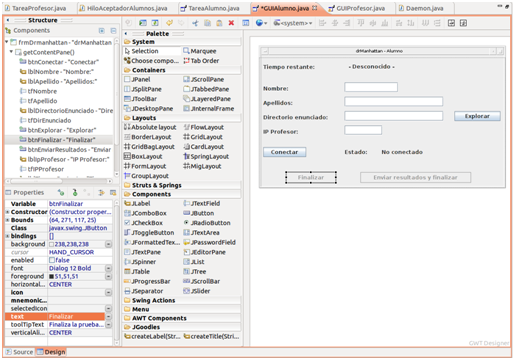
\includegraphics{implementacion/GWT2}
    \caption{Plug-in Google Web Toolkit}
    \label{fig:implementacion:GWT}
\end{figure}

\todo{comentar lo del google code}

Todo ello sobre el sistema operativo Ubuntu 9.10 de 32 bits y la versión de kernel 2.6.35.

\section{Creación de instaladores}
\label{sec:implementacion:instaladores}

Para que la aplicación pueda ser probada de un modo cómodo fuera del ambiente de desarrollo se hace necesaria la creación de instaladores. Esto se puede hacer, por ejemplo, con el comando \emph{dpkg} en sistemas Linux derivados de Debian, ya que con el se crear archivos .deb. En nuestro caso se han de crear dos instaladores, uno para la aplicación del profesor, y otro para la aplicación de los alumnos.
\newline

En el sistema de archivos, cada carpeta tiene su utilidad, conocida por todos, de modo que si, por ejemplo, queremos conocer los logs generados por alguna aplicación sabemos que hemos de buscar en /var/log/, /etc/ para los temas de configuraciones, etc.
\newline

Esto es interesante conocerlo para que los archivos que coloque nuestro instalador en el sistema, estén correctamente ubicados, de modo que se puedan localizar fácilmente, en caso de querer modificarlos o eliminarlos.
\newline


Por ejemplo, la aplicación del alumno, creará en los siguientes directorios, los siguientes ficheros:

\begin{itemize}

    \item {\bfseries /etc/rc2.d:}
    \begin{itemize}
        \item \emph{S88drManhattanDaemon}
    \end{itemize}

    Este fichero contiene un script muy simple que se encarga de iniciar en segundo plano el demonio. Los ficheros en este directorio se ejecutan cuando se entra al segundo nivel de ejecución, en el arranque del sistema.


    \item {\bfseries /usr/bin:}
    \begin{itemize}
        \item \emph{drManhattanAlumno.jar}
        \item \emph{drManhattanAlumno.sh}
        \item \emph{drManhattanDaemon.jar}
    \end{itemize}

    En este directorio se encuentran los ejecutables de las aplicaciones que pueden utilizar todos los usuarios.

    \item {\bfseries /usr/share/applications:}
    \begin{itemize}
        \item \emph{drManhattanAlumno.desktop}
    \end{itemize}

    En nuestro caso se ha utilizado un sistema Ubuntu con el entorno de escritorio GNOME, en ese directorio se guardan las entradas de cada aplicación que se puede ejecutar en GNOME, en archivos de texto dónde se especifica la ruta del ejecutable, el icono del programa, su versión, comentarios, etc.


    \item {\bfseries /usr/share/drManhattanAlumno/iconos:}
    \begin{itemize}
        \item \emph{icono.png}
    \end{itemize}

    Contiene los datos que no dependen de la arquitectura del sistema, imágenes, sonidos, etc.

    \item {\bfseries /usr/share/menu:}
        \begin{itemize}
            \item \emph{drManhattanAlumno}
        \end{itemize}

    Cada archivo localizado en este directorio contiene la información necesaria para que GNOME pueda crear una entrada en el menú despegable de aplicaciones.

\end{itemize}



Una vez que están definidos los archivos y el directorio dónde los ha de colocar el instalador, creamos una carpeta a modo de raíz en la que simulamos el árbol de directorios anterior. Por ejemplo, creamos la carpeta /home/usuario/deb, y dentro de ella creamos /home/usuario/deb/etc/rc2.d/, /home/usuario/deb/usr/bin/, etc y los archivos correspondientes.
\newline

Dentro de la carpeta raíz se ha de crear además de lo anterior, un directorio llamado \"DEBIAN\" con tres ficheros, "control", "postinst" y "postrm". En el primero se especifican las características del paquete y los otros dos se ejecutan justo después de instalar el paquete y justo después de desinstalarlo, respectivamente, en nuestro caso actualizan los menús desplegables para que aparezca o desparezca la aplicación.
\newline

Una vez que tenemos todo creado, cambiamos los permisos del directorio raiz y subdirectorios así:

\begin{center}
    \emph{chown root.root -R /home/usuario/deb/}
\end{center}

Después de esto, la orden para empaquetarlo en un fichero .deb es:

\begin{center}
    \emph{dpkg -b /home/usuario/deb /home/usuario/paquete.deb}
\end{center}

Para instalar, teniendo permisos de administrador:

\begin{center}
    \emph{dpkg -i /home/usuario/paquete.deb}
\end{center}


%Listado de pruebas
